\documentclass[journal, onecolumn, 11pt]{IEEEtran}
\usepackage{mathtools}
\usepackage{graphicx}
\usepackage{amssymb}
\usepackage{amsmath}
\usepackage{pythonhighlight}
\usepackage[utf8]{inputenc}
\usepackage{fancyhdr}
\usepackage{pythonhighlight}
\usepackage{changepage}
\usepackage{slashbox}
\usepackage{floatrow}
\usepackage{listings}
\usepackage[hidelinks]{hyperref}
\usepackage{fontawesome}
\usepackage{caption}
\usepackage{subcaption}
\usepackage{cleveref}
\usepackage[style=ieeetran,style=numeric,sorting=none]{biblatex}
\addbibresource{references.bib}
\usepackage{color} 
\usepackage[english]{babel}
\usepackage{amsthm}
\usepackage{makecell}
\usepackage{diagbox}
\newtheorem{theorem}{Theorem}

\author{Kutay Ugurlu}
\title{Analysis of Deep Convolutional Neural Network for Inverse Problems in Imaging
}
\begin{document}
\maketitle
\tableofcontents
\listoffigures
\listoftables
\clearpage

\section{Introduction}
In this term project report, the study \textit{Analysis of Deep Convolutional Neural Network for Inverse Problems in Imaging} by Jin \textit{et al.} \cite{FBPConvNet} is going to be reviewed, the results are going to reproduced and the experiments are going to be conducted using another dataset which is going to be formed by hand. 
\\
\\
The authors of the paper propose a convolutional neural network architecture mainly for the inverse problem of computerized tomography(CT) problems, while they stress that the proposed method is available for all normal-convolutional inverse problems. The study aims reconstructing the image from lower views by direct inversion followed by a convolutional neural network, more specifically a U-Net \cite{ronneberger2015u} based architecture. Starting from the observation that the normal operator $H^\ast H$, where $H^\ast$ is the adjoint operator of H that satisfies the relation $\langle f,H^\ast g \rangle = \langle Hf,g \rangle$, that appears as a forward model in a set of inverse problems, the authors investigate the relationship between the CNN models and the iterative optimization models.  

\section{Theory}

\subsection{Shift-invariant Normal Operator}

To define a shift-invariant normal operator, the authors made the following definitions for the continuous domain: 
\begin{enumerate}
    \item \textit{Isometry:} An isometry $T$ is a linear operator such that $T^\ast T {f}(x) = f(x)$
    \item \textit{Multiplication:} A multiplication $M_m$ is a linear operator such that $M_m{f}(x) = m(x)f(x)$ where $m(x)$ is a continuous and bounded function.  
    \item \textit{Convolution:} A convolution $H_h$ is a linear operator such that $H_hf = \mathcal{F}^\ast M_{\hat{h}} \mathcal{F} f$ where $\mathcal{F}$ is the Fourier transform and $\hat{h}$ is the Fourier transform of h. 
    \item \textit{Reversible Change of Variables:} A reversible change of variables $\Phi_\psi: L_2(\Omega_1) \rightarrow L_2(\Omega_2)$ is a linear operator such that $\Phi_\phi f = f(\phi(.))$ for some $\phi: \Omega_2 \rightarrow \Omega_1$ and such that its inverse exists. That is, it is a linear operator that represents the same function via a reversible domain transformation, such as Cartesian to Polar coordinate transformation. 
\end{enumerate}

\begin{theorem}
    If an operator is in the form $H = TM_m{\Phi_\phi}^{-1}\mathcal{F}$, then normal operator $H^\ast H$ represents a convolution operation with $|det J_\phi| M_{\Phi_\phi |m|^2}$
    \label{thrm:Theorem1}
\end{theorem}
where $J_\phi$ is the Jacobian matrix.

\subsection{Forward Model of X-Ray CT Problem}
The main focus of the paper is reconstructing the X-ray CT image from low-view projections. When we consider the forward model as the 2 dimensional X-Ray Transform $R: L_2()\mathbb{R}^2) \rightarrow L_2([0,2\pi) \times \mathbb{R})$, also known as Radon Transform, we can express it using Fourier Slice Theorem as follows: 
\begin{equation}
    R = T {\Phi_\phi}^{-1} \mathcal{F}
    \label{eq:RadonTransform}
\end{equation}

\begin{figure}[h]
\centering
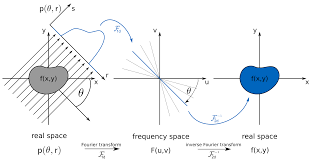
\includegraphics[width=0.8\textwidth]{images/images.png}
\caption{Illustration of reconstruction via Radon Transform \cite{radonimg}}\label{fig:radonimg}
\end{figure}

where the coordinate transformation operation is defined as conversion from Cartesian to polar coordinates and $T$ is inverse Fourier transform. The operation expressed by Eqn. \ref{eq:RadonTransform} takes the Fourier transform of the image, express the resultant signal in polar coordinates and takes the inverse Fourier transform. This process is illustrated in Figure \ref{fig:radonimg}. Theorem \ref{thrm:Theorem1} states that $R^\ast R$ is a convolution with $\frac{1}{||w||}$ where w is the frequency variable for the 2D Fourier transform. 

\subsection{Direct Inversion}

One may apply direct inversion methods to solve the inverse problem of tomography, \textit{i.e.}, obtaining the image from measurements. The problem can be formulated as $g=Hf$ where $H$ is a normal convolutional operator. According to \cite{FBPConvNet}, the solution can be obtained by direction inversion in two ways as follows: 

\begin{align}
    f &= W_h H^\ast g \label{eq:inv1}\\
    f &= H^\ast T M_h T^\ast g \label{eq:inv2}
\end{align}

where $W_h$ in \Cref{eq:inv1} is the convolution operator with $\frac{1}{|det J_\phi|\Phi_\phi|m(w)|^2}$ and $M_h$ is $\frac{1}{|det J_\phi||m(w)|^2}$. The physical interpretation behind these equations can be considered as follows: The operation in \Cref{eq:inv1} corresponds to the deconvolution in the reconstruction space, whereas \Cref{eq:inv2} corresponds to a filtering operation in Fourier domain followed by a back- projection, if $T$ is Fourier transform. 

\subsection{Iterative Inversion}

There also exist iterative approaches to solving inverse problems and they are formulated as follows: 

\begin{equation}
    \operatorname*{argmin}_a ||y-HWa||_2^2 + \lambda ||a||_1 
\end{equation}

where $x = Wa$ and $a$ is a sparse representation of x in a domain where x is transformed to by $W$.

\section{Proposed Method: FBPConvNet}

The authors state that the filtering and pointwise linearity operations in the iterative reconstruction methods may suggest that CNNs may be a good fit for the solution of the inverse problems. 
\\
\\
The approach simply consists of applying a direct inversion method to the measurements (sinograms in CT case) by Matlab's \texttt{iradon} function and feed the resultant projections to the CNN to train the network to learn the mapping between the back projected measurements and suitable ground truth images. 
The authors explain the reason for using a direct inversion method, instead of following an end-to-end neural net training approach between measurements and ground truth images as follows: 
By projecting the measurements to image domain, the learning is greatly simplified due to the fact that the network does not have to learn the coordinate transformation between Cartesian and Polar space. Since, filtered back projection encapsulates this operation and the physical information about the forward model. 

\subsection{Neural Network Model}

The design of the proposed network was based on U-Net. The modified architecture is illustrated in \Cref{fig:Unet}.

\begin{figure}[h]
\centering
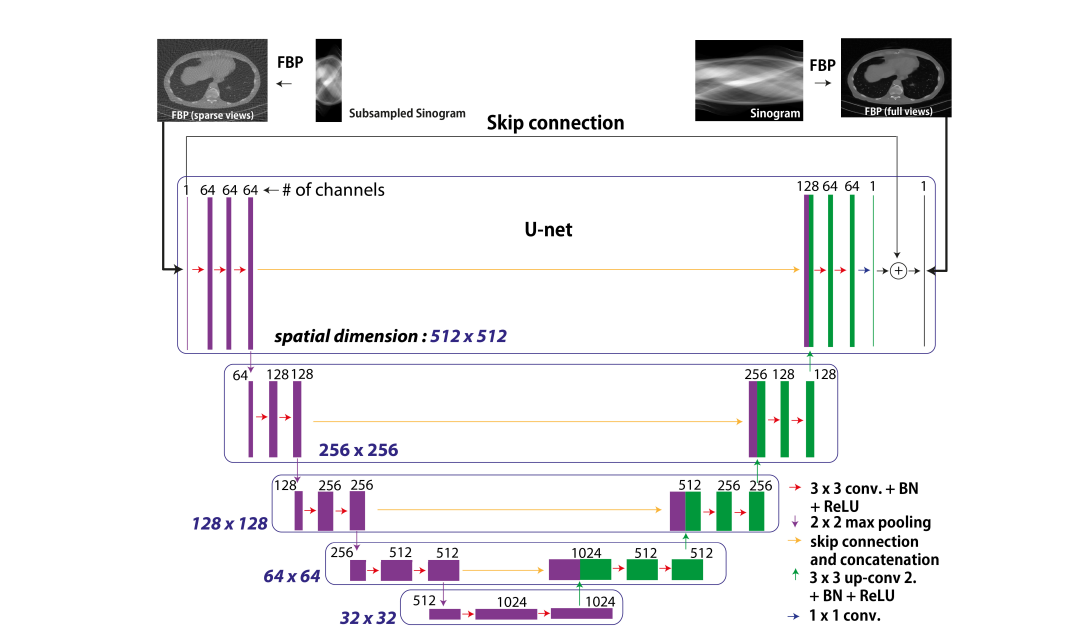
\includegraphics[width=0.8\textwidth]{images/unet.png}
\caption{Modified U-Net Architecture}\label{fig:Unet}
\end{figure}

The authors summarized the reasons for basing their architecture on U-Net as follows: 
\begin{itemize}
    \item \textit{Multilevel Decomposition:} The use of pooling kernels with different sizes help the network effectively invert $H^\ast H$. 
    \item \textit{Multichannel filtering:} The convolutional kernels have the ability to make arbitrary combinations of channels, analogous to wavelet subbands in ISTA or split variables in ADMM. 
    \item \textit{Residual Connection:} In addition to the original U-Net work, the authors added a skip connection between the input and output, allowing the network to learn the difference between the input and output. These connections have significant improvement in overcoming the gradient vanishing problem. 
    \item \textit{Last Layer:} The last layer of the network is replaced with a convolution layer, since the original U-Net implementation has 2 channels: foreground and background. 
\end{itemize}

\subsection{Experiments}

Jin \textit{et al.} begin the reconstruction via full view sinogram from both real and simulated data. Then the reconstruction is performed on the subsampled sinogram. This type of procedure holds an important place in human imaging because lowering the views lower the radiation dose received by the patient. The full-view filtered back projection data is used as ground truth images, rather than the actual image, since the authors believe that this is a more realistic setting in practice and the oracle information will never be available in CT. 


\subsection{Training Procedure}

The sample size of the train and test splits of the datasets are given in \Cref{tab:dataset}. 

\begin{table}[h]
    \centering
        \caption{Samples for Datasets}
\begin{tabular}{|c|c|c|c|}
\hline 
\diagbox{Dataset}{Split} & \makecell{Training Data} & \makecell{Test Data} & Total \\ 
\hline 
Synthetic (Ellipsoidal) & 475 & 25 & 500 \\ 
Real (Biomedical) & 327 & 25 & 352 \\ 
\hline 
\end{tabular}
    \label{tab:dataset}
\end{table}

The CNN part of the network is trained with pairs of low view and full view FBP images. To reduce the overfitting, data augmentation is realized by mirroring the images in both vertical and horizontal directions. To prevent the cost function from diverging, the gradient clipping procedure is applied. The hyperparameters for state-of-the-art TV reconstruction \cite{TV} for comparison study is set experimentally by hand. 

\section{Results and Discussion}

\subsection{Reconstruction Performance Metrics}
The authors use SNR as a quantitative metric. The SNR of the reconstruction $\hat{x}$ with the ground truth image $x$ is given by \Cref*{eqn:SNR}.

\begin{equation}
    SNR = \operatorname*{max}_{a,b \in \mathbb{R}} \frac{||x||_2}{||x - a\hat{x} + b||_2}
    \label{eqn:SNR}
\end{equation}

\subsection{Sample Reconstructions}

\begin{figure}[h]
\centering
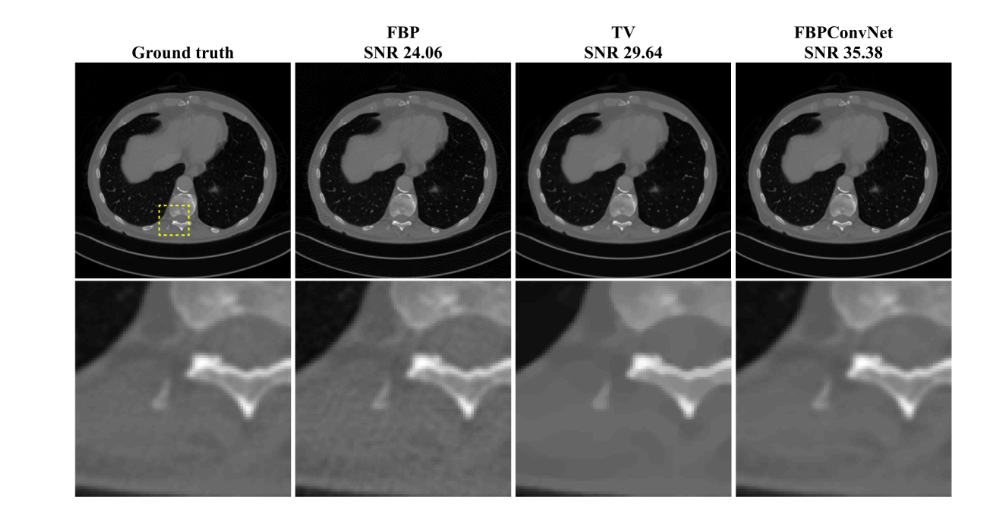
\includegraphics[width=0.8\textwidth]{images/results1.png}
\caption{Reconstructed images of biomedical dataset from 143 views}\label{fig:res1}
\end{figure}

\begin{figure}[h]
    \centering
    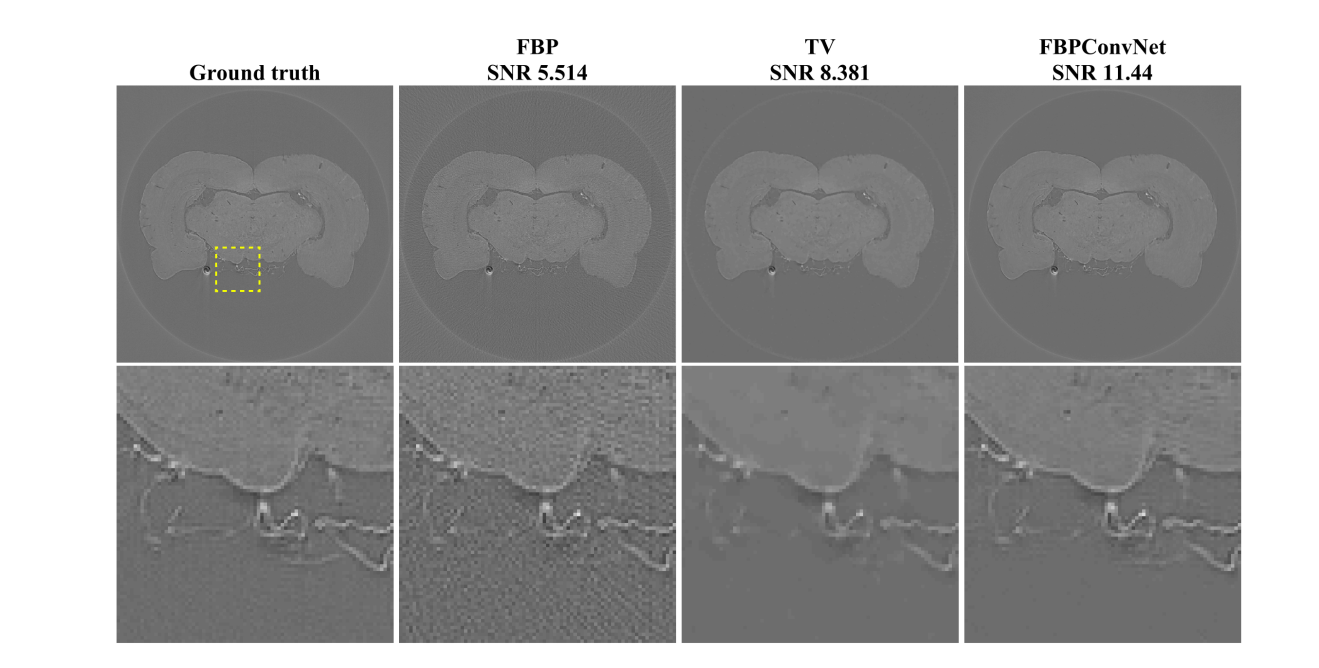
\includegraphics[width=0.8\textwidth]{images/results2.png}
    \caption{Reconstructed images of experimental dataset from 145 views}\label{fig:res2}
\end{figure}

The results of the experiments showed that the choice of CNN for the set of inverse problems where the forward model is convolution is suitable. In both \Cref*{fig:res1} and \Cref*{fig:res2} the denoising performance of the FBPConvNet against back projection can be observed qualitatively. The proposed method yields compelling results in both real and synthetic data. It outperformed when the state-of-the-art iterative reconstruction methods. Once the training is finished, the computation time for an image is computed to be under a second. 

\printbibliography

\end{document}